    %\setcounter{partie}{0} % Pour s'assurer que le compteur de \partie est à zéro dans les corrigés
    \phantom{rrr}

    \begin{multicols}{2}
        Sur la figure ci-dessous :
        \begin{itemize}
            \item Les points $S$, $D$, $B$ sont alignés.
            \item Les points $S$, $C$, $A$ sont alignés.
        \end{itemize}
        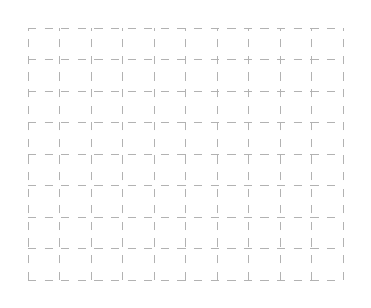
\begin{tikzpicture}[scale=0.4]
            \draw[help lines, color=black!30, dashed] (0,0) grid (10,8);
            \coordinate (O) at (1,1);
            \coordinate (C) at (4,1);
            \coordinate (S) at (9,1);
            \coordinate (D) at (9,5);
            \coordinate (B) at (9,7);
            \tkzDrawSegment[ultra thick](O,S);
            \tkzDrawSegment[ultra thick](O,B);
            \tkzDrawSegment[ultra thick](B,S);
            \tkzDrawSegment[ultra thick](C,D);
            \tkzLabelPoints[above right](B);
            \tkzLabelPoints[below left](O);
            \tkzLabelPoints[below right](S);
            \tkzLabelPoints[right](D);
            \tkzLabelPoints[below](C);
        \end{tikzpicture}

        \columnbreak
        Justifier que $(AB)$ et $(CD)$ ne sont pas parallèles.

        \smallskip
        {\color{red} $\dfrac{SC}{SA}=\dfrac{5}{8}=\dfrac{15}{24}$ et $\dfrac{SD}{SB}=\dfrac{4}{6}=\dfrac{16}{24}$ donc $\dfrac{SC}{SA}\neq \dfrac{SD}{SB}$

        \smallskip
        Si $(AB)$ et $(CD)$ étaient parallèles, les rapports seraient égaux.

        D'après la contraposée du théorème de Thalès, $(AB)$ et $(CD)$ ne sont pas parallèles.
        }
    \end{multicols}

